\documentclass[12pt]{article}
\usepackage{amsmath}
\usepackage{graphicx}
\usepackage{fancyhdr}
\usepackage[margin=1in]{geometry}
\usepackage{url}
\usepackage{float}
\usepackage{todonotes}
\usepackage{fixltx2e}
\usepackage{gensymb}
\usepackage{enumitem}
\usepackage{textpos}
\usepackage{appendix}
\usepackage{color}
\usepackage{tabu}
\usepackage{listings,xcolor}
\usepackage{textcomp}
\usepackage{pdfpages}
\usepackage{enumitem}
\usepackage{wrapfig}
\usepackage{array}
\usepackage{libertine} \usepackage[libertine]{newtxmath}
\newcolumntype{L}{>{\arraybackslash}m{5in}}
\setlength\extrarowheight{2pt}
\pagestyle{fancy}
\usepackage[font=small,labelfont=bf,tableposition=top]{caption}
\fancyhf{}
% Header and footer
\fancyhead[L]{ENGR 4595}
\fancyhead[C]{Final Report}
\fancyhead[R]{Group 2}
\fancyfoot[R]{Page \thepage}
\renewcommand{\headrulewidth}{0.4pt}
\renewcommand{\footrulewidth}{0.4pt}
\newcommand*{\everymodeprime}{\ensuremath{\prime}}
\begin{document}
\begin{titlepage}

\newcommand{\HRule}{\rule{\linewidth}{0.5mm}} % Defines a new command for the horizontal lines, change thickness here

\center % Center everything on the page
 
%----------------------------------------------------------------------------------------
%	HEADING SECTIONS
%--------------------------------------------------------------------s--------------------

\textsc{\LARGE Laurentian University}\\[1.5cm] % Name of your university/college
\textsc{\Large Capstone}\\[0.5cm] % Major heading such as course name
\textsc{\large ENGR-4595}\\[0.5cm] % Minor heading such as course title

%----------------------------------------------------------------------------------------
%	TITLE SECTION
%----------------------------------------------------------------------------------------

\HRule \\[0.4cm]
{ \huge \bfseries Final Report: Robot Drive System Redesign}\\[0.4cm] % Title of your document
\HRule \\[1.5cm]
 
%----------------------------------------------------------------------------------------
%	AUTHOR SECTION
%----------------------------------------------------------------------------------------

\begin{minipage}{0.4\textwidth}
\begin{flushleft} \large
\emph{Submitted by Group 2:}\\
Dyson Chambers \textsc{} \\
Dominic Girard \textsc{} \\
Christopher Gravelle \textsc{} \\
Jacob Lachapelle \textsc{} \\
Genevi\`{e}ve Rodrigue \textsc{}
\end{flushleft}
\end{minipage}
~
\begin{minipage}{0.4\textwidth}
\begin{flushright} \large
\emph{For project client:} \\
Penguin ASI\\
Regional Road 55\\
Naughton, ON % Supervisor's Name
\end{flushright}
\end{minipage}\\[4cm]


% If you don't want a supervisor, uncomment the two lines below and remove the section above
%\Large \emph{Author:}\\
%John \textsc{Smith}\\[3cm] % Your name

%----------------------------------------------------------------------------------------
%	DATE SECTION
%----------------------------------------------------------------------------------------

{\large April 26, 2016}\\[3cm] % Date, change the \today to a set date if you want to be precise

%----------------------------------------------------------------------------------------
%	LOGO SECTION
%----------------------------------------------------------------------------------------

%\includegraphics{Logo}\\[1cm] % Include a department/university logo - this will require the graphicx package
 
%----------------------------------------------------------------------------------------

\vfill % Fill the rest of the page with whitespace
\end{titlepage} 

% front matter goes here
\tableofcontents
\newpage
\listoftables
\newpage
\listoffigures
\newpage
% body material goes here
\section{Introduction}
Penguin ASI is a robotics firm engaged in the development of automation strategies for the mining industry and the development of telerobotic systems to work in extreme and hazardous environments. As the use of automated technology becomes more prevalent in the mining industry there comes a need to develop a telecommunications network. In order to prevent the need to retrofit an existing mine with a communications network, Penguin had developed an optical communications range extender and mounted it on a teleoperated, mobile platform to be able to relay the signals. The first iteration of this platform had some issues with its design that Penguin had wished to resolve in a second iteration prototype. In order to produce a functional prototype all issues with the previous version must have been addressed, and the robot must have been able to achieve certain functional requirements laid out by the client, Penguin ASI.  
\subsection{Problem Statement}
The initial communications robot produced by Penguin ASI had displayed many issues affecting its performance that needed to be addressed. Its operating environment was intended to include traversal through wet and rough terrain, which required all drive components to be sealed against water and dirt. To seal the original drive boxes gasket maker was used, but proved to be inadequate and allowed water to enter the drive box as seen in Figure~\ref{fig:inside_drive_box_orig}. Secondly, the drive box travel was not limited to $\pm$30\degree rotation initially, and a spring system was implemented as a temporary solution. Only two, 746\,W motors were used, and after testing were deemed insufficient to drive the vehicle and payload up hills of a 20\% grade. Furthermore, each motor drove four wheels and transmitted power through a long chain extending the length of the vehicle as seen in Figure~\ref{fig:interior_orig}. The length and complexity of the chain driven system introduced many modes of failure, slapped the bottom of the vehicle during skid steer operation and change of direction, and did not have an adequate tensioning device. 
\begin{figure}[h]
\centering
\begin{minipage}{0.45\linewidth}
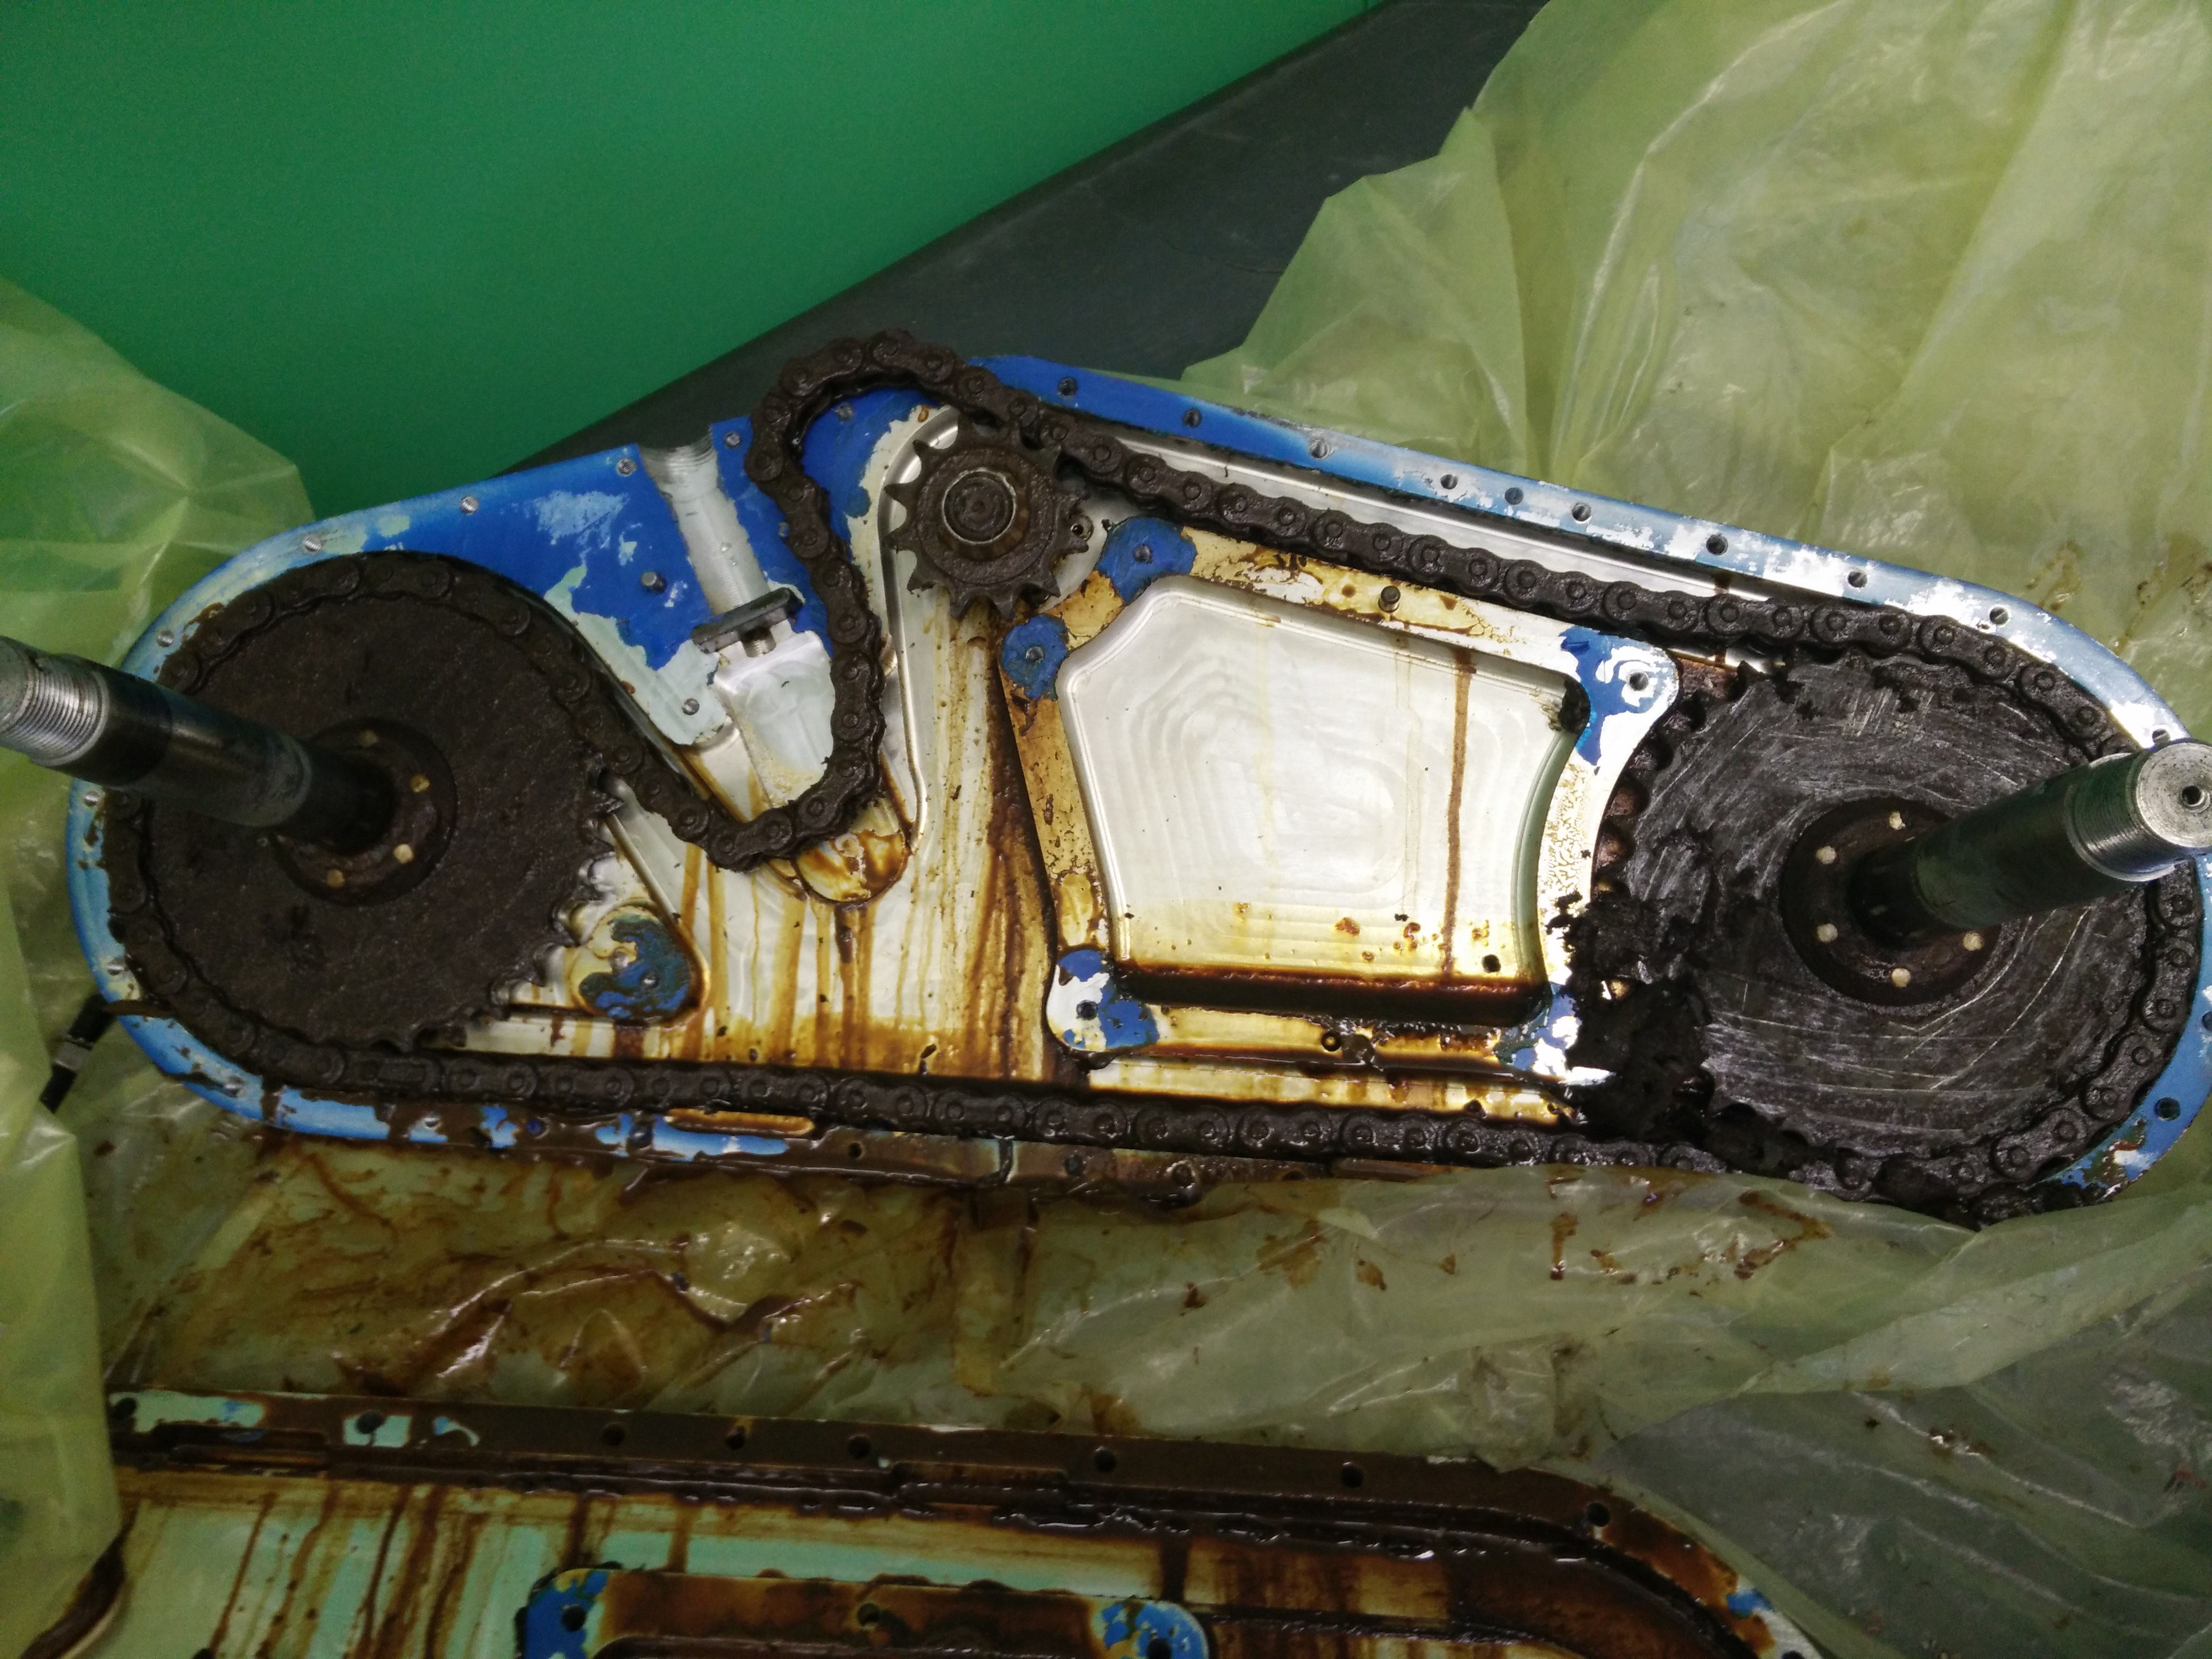
\includegraphics[width=\linewidth]{./images/inside_drive_box_orig}
\caption{Original Drive Box Interior Demonstrating Improper Sealing}
\label{fig:inside_drive_box_orig}
\end{minipage}
\begin{minipage}{0.45\linewidth}
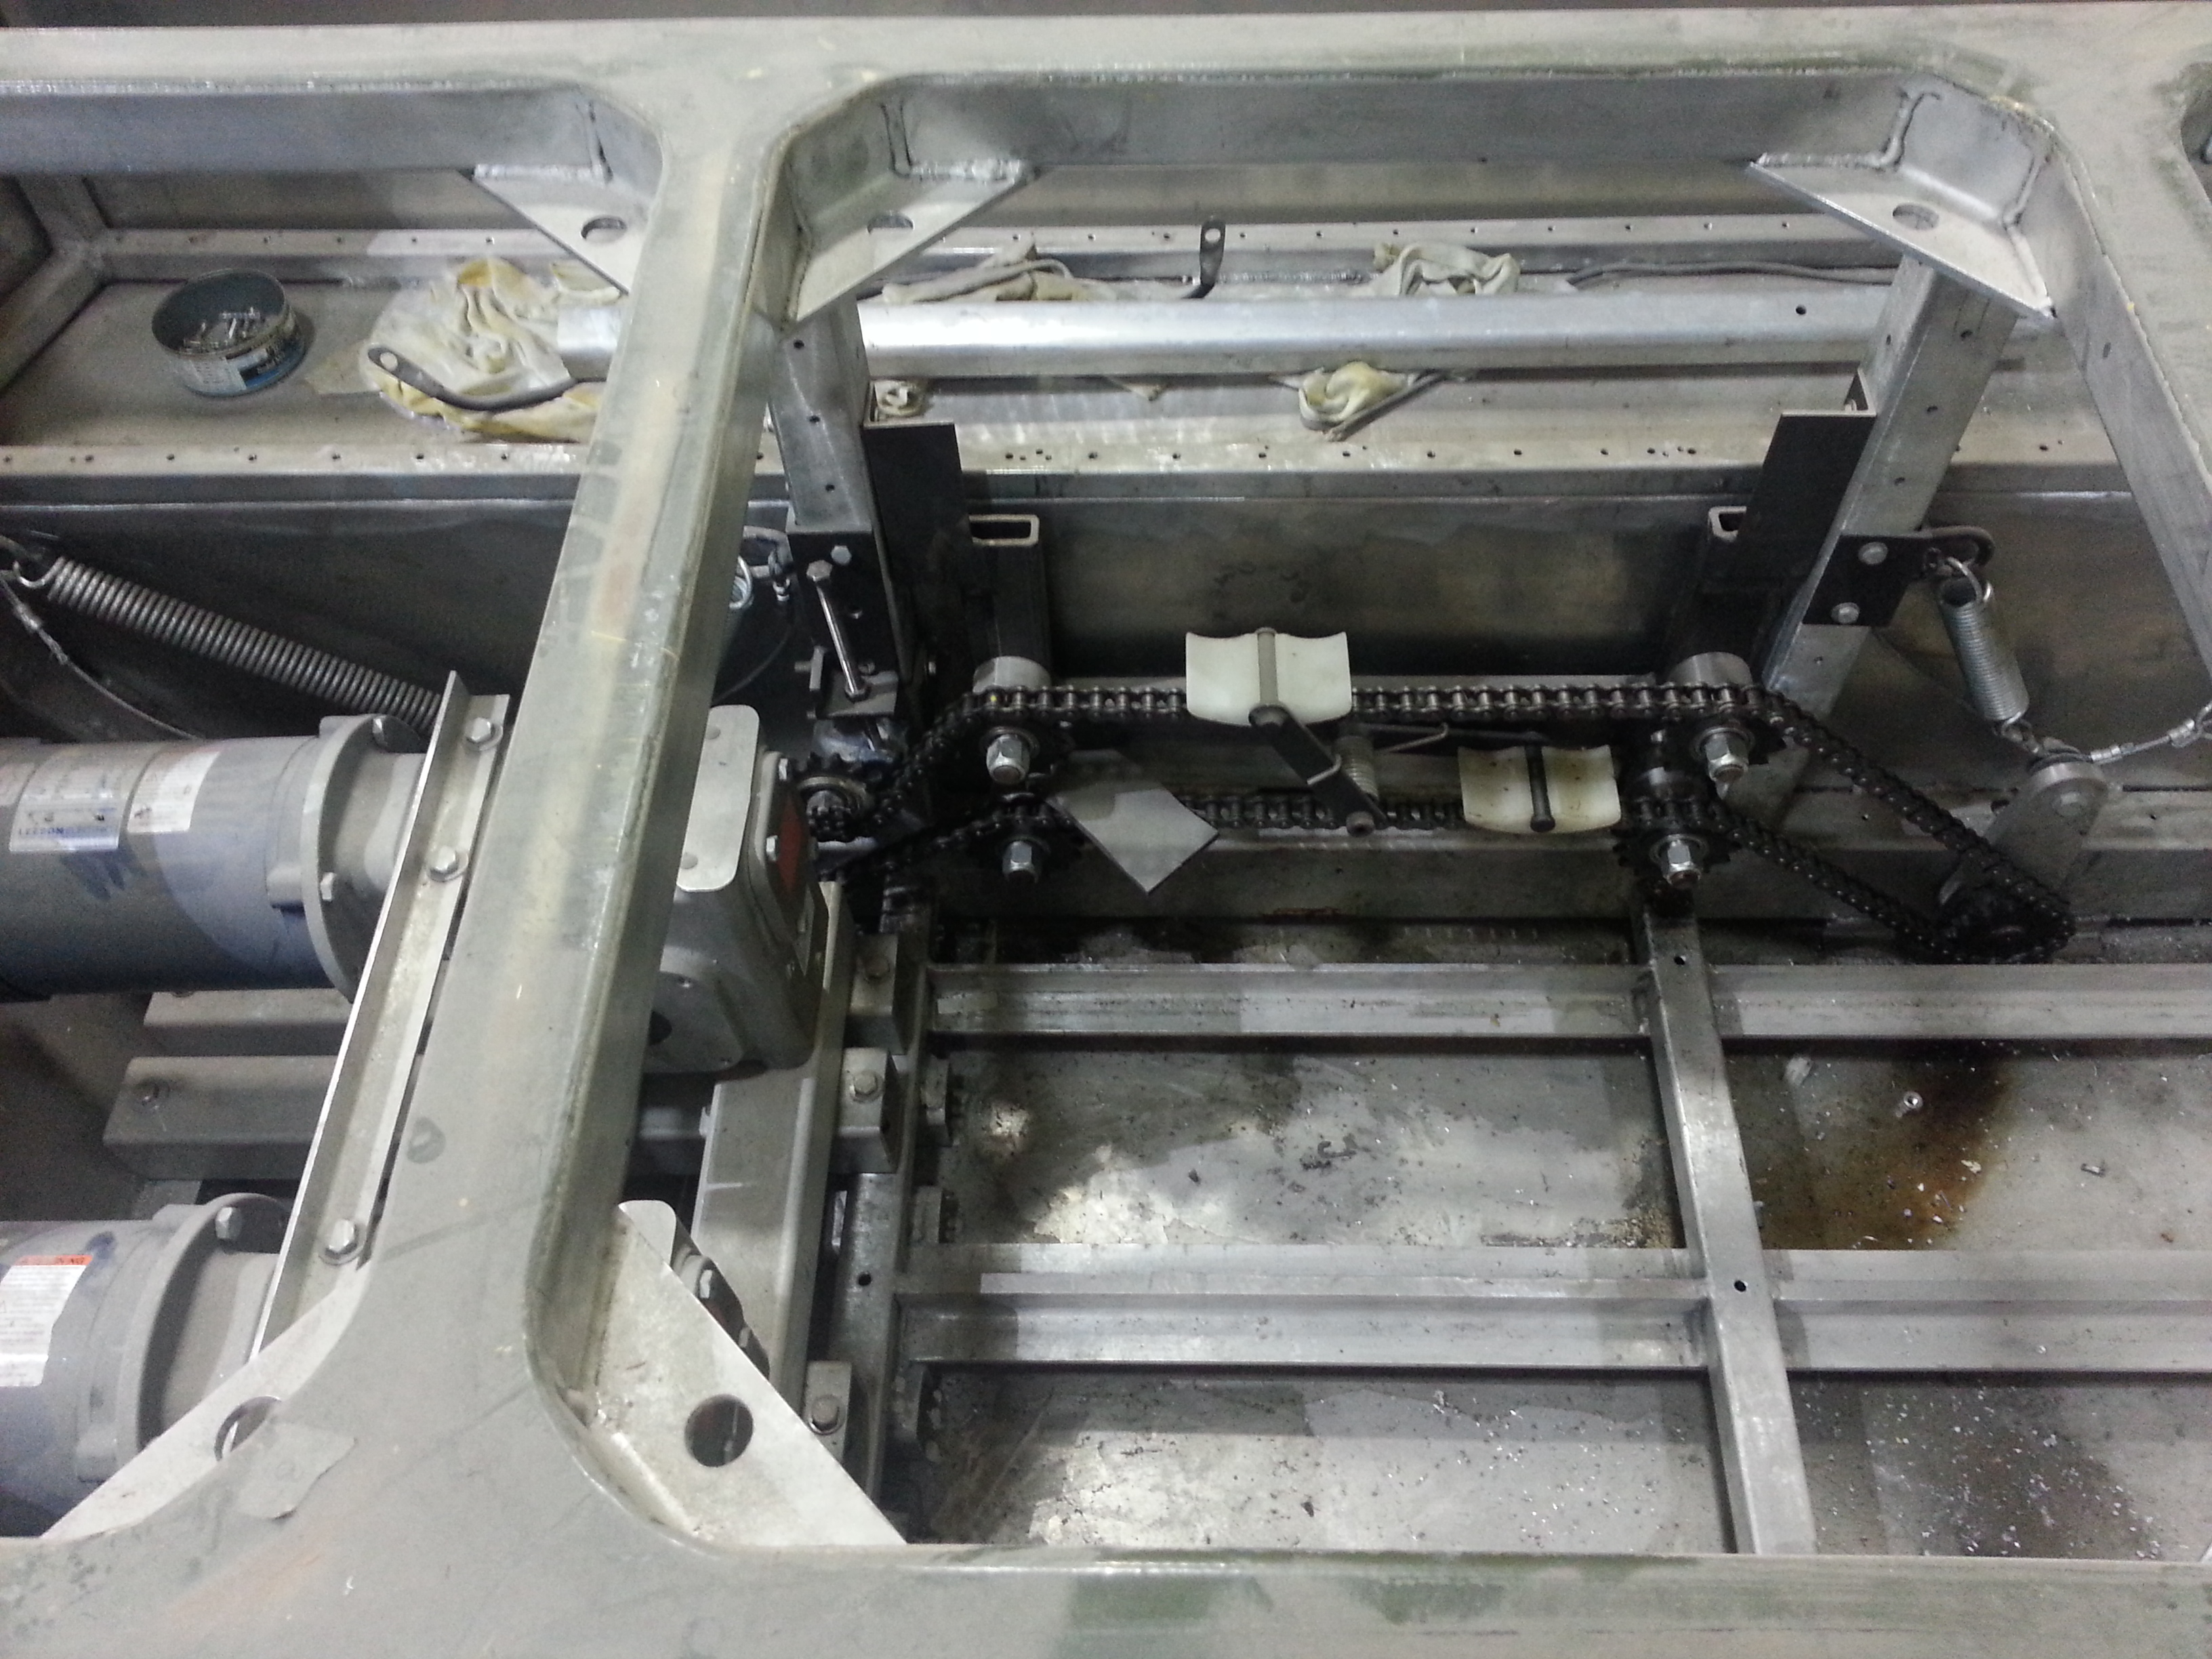
\includegraphics[width=\linewidth]{./images/interior_orig}
\caption{Chain Driven System Inside Vehicle Body}
\label{fig:interior_orig}
\end{minipage}
\end{figure}

The disassembly of the original driveboxes was difficult and it was observed that there was no way to determine oil levels without opening them up. Also, under skid steer operation it was reported that the drive boxes underwent significant deflection which was not desireable. Each drive box was chain driven, however there was no method to determine the chain tension, which was problematic and was suspected to be the cause of premature failure of chains. Other components that were failing included radial bearings used on the drive shafts and wheel shafts. After opening the drive boxes it was observed that these radial bearings were paired with a single taper roller bearing and it was suspected that the cause of failure was the axial loading on the radial bearing. 
\subsection{Functional Requirements}
Overall the vehicle was able to drive and maneuvre with limited capabilities, however it was in the interest of the client to address these issues for a redesign of the product. In order to meet the needs of the client a list of requirements for the final design were agreed upon. The requirements were broken down into six main categories, with each highlighting the necessary functionality for the redesign of the communications robot. 
\subsubsection{Power}
The vehicle was to be fully battery powered using six EV Traction Dry Cell Industrial Battery Blocks. To drive the vehicle, four 746\,W DC motors were provided by Penguin ASI. The drive time of the vehicle was to exceed one hour at peak operating conditions, and the batteries were to be seated in the vehicle to provide clearance between battery terminals and frame components.
\subsubsection{Operating Conditions}
The vehicle was to be used in aboveground and underground mining applications, and as such would be subject to varying temperatures, however the client had specified the need to operate primarily in 2\,\degree C. The vehicle also needed to be able to climb and descend a maximum grade of 20\% and have every component sealed from external water.
\subsubsection{Size and Weight}
All components of the vehicle were to remain within the dimensions of the frame with the exception of the wheels. The robot needed to be able to carry a payload of 230\,kg in addition to its own weight, and be able to reach a top speed of 3\,km/h under these conditions.
\subsubsection{Interfacing}
Penguin ASI had specified the need to reuse the frame from the existing robot, however minor frame modification were permitted. Motor interfacing needed to be done using a Roboteq controller, and battery charging was to be carried out by employees at Penguin. The redesign of the vehicle needed to ensure that that existing communications devices and telescoping arms could still be mounted on the upper platform of the frame, and that space be left in the wings of the vehicle to accomodate electrical components.
\subsubsection{Robot Control}
The motors on each side of the vehicle were to be controlled independently. A Roboteq controller was to be used, and appropriate voltage limits were to be programmed into the controller to prevent damaging the motors. For testing purposes, the use of a laptop to and joystick to control the motors was permitted. The implementation of wireless control was to be carried out by Penguin employees upon the successful demonstration of an operable vehicle.
\subsubsection{Care and Maintenance}
All new components were to be designed with the intent of improving functionality and maintainability. It was desired that all components be easy to assemble/disassemble, internal components be easily accessible, and grease nipples be incorporated to grease bearings. Furthermore, a means to check belt tension was to be incorporated in the final design.       
\input{design_alternatives}
\input{project_management}
\input{final_design}
\input{technical_specifications}
\input{final_budget}
\section{Testing}
\subsection{Initial Build}
While the first drive box was being manufactured, the code for the controller was tested with the motors and the batteries as a dry run to ensure that the program functioned as required, with a top speed of 3 km/h. The controller was tested by adjusting the voltage that the controller provided to the motors and both direction of rotation. After the completion of one assembled drive box it was placed into the chassis of the robot with the motor and the controller. The assembly was then tested without wheels or loading to ensure that all components within the drive box worked together and that no rubbing or undesired out comes were to happen. During this testing all components operated correctly and was able to handle the maximum rotation to achieve the desired speed of 3 km/h. During the manufacturing of the initial drive box some design changes were brought up that would help both improve our design along with decrease the manufacturing time of some components. The 1/4" aluminum plate that was required on the back plate was dropped and the hole was filled on the first 1" plate to enclose the drive box. The rear hubs were also changed to ensure that sealing would be achieved at the back. The rear hubs design also changed to reduce machining time and to make the assembly easier for inserting both the shaft seals and bearing races. A flexible Lovejoy coupling was implemented instead of the custom one that was proposed to allow mounting of the output shaft to the reduction shaft a simpler task during assembly and to help with any misalignment that may have occurred between the two during the frame modifications. The cut outs on the 1" rear and front drive boxes were changed to decrease the stress concentrations at the corners and to reduce the amount of machining time for each plate. For pivot the numbers of fasteners used to mount to the drive box was reduced from 12 bolts to 10 since it was unnecessary to have that many and it decreased the amount of fasteners used in the assembly, while reducing machining time. A snap ring grove was added to the output shaft to prevent the coupling from sliding back on the shaft and losing the connection to the reduction shaft.

\subsection{Final Build}
When the final build was completed it was tested using the same program and controller as the initial test and the assembly worked accordingly. The improvements made allow us to cut the amount of machining time used and allowed for an easier assembly while keeping the same desirable outcomes of the design. In the final testing done by us the controller was connected to two drive boxes and running them under no loads to ensure that but operated correctly together. The controller and the assemblies of the drive boxes work as designed for both the forward and reverse directions of rotation.

\subsection{DFMEA}

Design Failure Modes and Effects Analysis was performed for the entire robot. Critical points of failure were identified as the wheel shaft and drive box. The analysis is presented in full in Appendix~\ref{sec:dfmea}.

% back matter goes here


\end{document}